In this part, we introduce an approach of meta reinforcement learning for solving the problem of exploration, which is named model agnostic exploration with structured noise (MAESN) [12]. With the method an agent can be enabled to explore more effectively in new situations based on prior experience.
\subsection{overview}
It is well-known that exploration is a critical task in reinforcement learning. As the practical tasks are becoming more and more complex, the prior proposed exploration strategies, such as information gain [13] or state visitation bonuses [14], perform not as well as expected, especially for multi-task problems. The approach model agnostic exploration with structured noise (MAESN), that has a combination of structured stochasticity with MAML, offers exploration strategies that are informed by prior knowledges and are more effective than random action-space noise.

The core idea of this gradient-based algorithm is to use prior experience both to initialize a policy and to learn a latent exploration space, by which the structured stochasticity injected policy can produce more effective exploration strategies on new task.

\subsection{ Meta-Learning Latent Variable Policies}
The conventional action distribution in reinforcement learning is written as $\pi_{\theta}(a\mid s)$, which possesses no property of temporally coherent randomness throughout the trajectory because it is independent for each time step. To address this problem we introduce latent variables $Z$. 
\begin{figure}[H]
	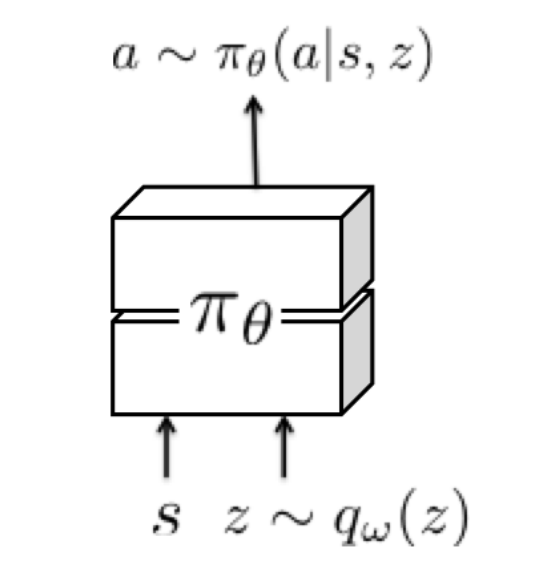
\includegraphics[scale=0.6]{MAESN_01.PNG}
	\centering
	\caption{latent variables}
	\label{MAESN}
\end{figure}

 We condition the policy on random variables, which are randomly drawn from a learned latent distribution. As the latent variable is sampled once per episode, the structured stochasticity in the process of exploration can be certainly ensured. The latent variable conditioned policy is represented as $\pi_{\theta}(a \mid s, z)$, where $z \sim q_{\omega}(z)$ and $q_{\omega}(z)$ is latent variable distribution with parameter $w$. 

Our aim is to meta-train the latent variable conditioned policy to generate coherent exploration strategies that perform faster adaptation on new tasks. Briefly, we jointly learn a set of policy parameters $\theta$ and the parameters of latent space distribution $w$, such that a policy gradient adaptation step can lead to maximal rewards.

\begin{figure}[H]
	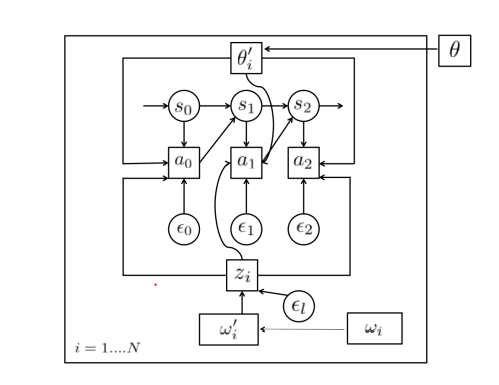
\includegraphics[scale=0.7]{MAESN_02.PNG}
	\centering
	\caption{Computation graph for MAESN}
	\label{MAESN}
\end{figure}

The objective of meta-training consists of not only sum of rewards under the post update parameters, but also the KL-divergence between the per-task pre-update distributions $q_{\omega_{i}}\left(z_{i}\right)$ and a prior $p(z)$, which ensures a effective structured exploration.
The full meta-training problem can be stated mathematically as:

\begin{figure}[H]
	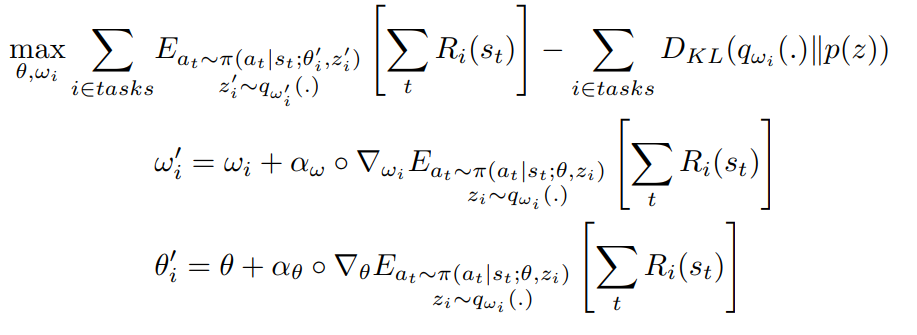
\includegraphics[scale=0.48]{MAESN_03.PNG}
	\centering
	\caption{meta-training procedure}
	\label{MAESN}
\end{figure}

The structure of training here is the same as the one in MAML, where two-level gradient is contained. The inner policy gradient is performed on the variational parameters for each task to get post-update parameters $\theta_{i}^{\prime}, \omega_{i}^{\prime}$, and then a meta-gradient is conducted to obtain $\theta$,$\omega_{0}$,$\omega_{1}$,...,$\omega_{N}$.

\begin{figure}[H]
	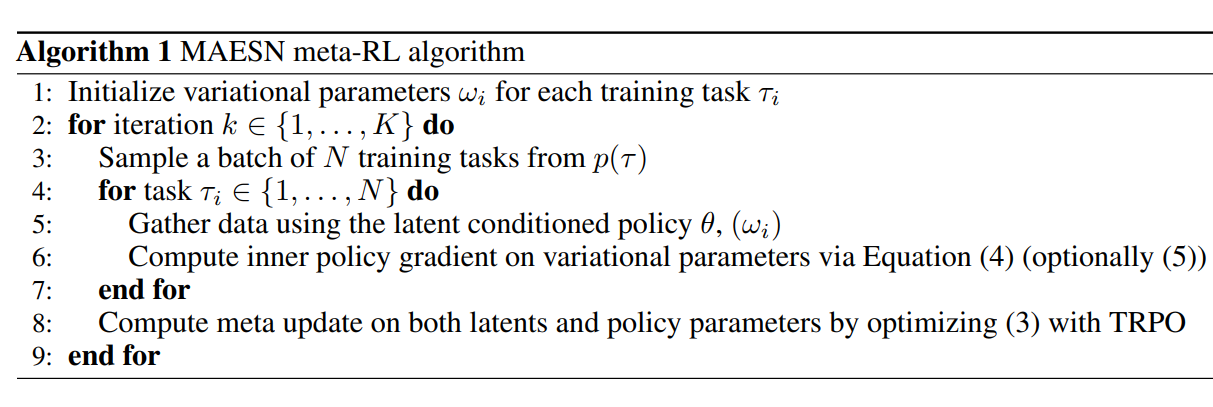
\includegraphics[scale=0.34]{MAESN_04.PNG}
	\centering
	\caption{MAESN algorithm}
	\label{MAESN}
\end{figure}

During the meta-train the sum of expected task rewards over all tasks is maximized and on the countrary the KL-divergence of pre-update distributions $q_{\omega_{i}}\left(z_{i}\right)$
against the prior$p\left(z_{i}\right)$ is minimized.
According to training procedure we can understand MAESN as augmentation of MAML with a latent space to inject structured noise.

Wenn adapting to new task, the variational parameters $\omega_{i}$ used during meta-training are not suitable anymore. $\omega$ is adapted by using the policy gradient via backpropagation on the RL objective:
$$
\max _{\omega} E_{a_{t} \sim \pi\left(a_{t} \mid s_{t}, \theta, z\right), z \sim q_{\omega}(.)}\left[\sum_{t} R\left(s_{t}\right)\right]
$$
In the inner loop, backpropagate through the sampling operation is needed to compute the gradients with respect to $\omega$, using either likelihood ratio or the reparameterization trick:

$$
\nabla_{\omega} \eta=E_{a_{t} \sim \pi\left(a_{t} \mid s_{t} ; \theta, z\right)}\left[\nabla \sim q_{\omega}(\cdot)^{ }\left[\nabla_{\omega} \log q_{\omega}(z) \sum_{t} R\left(s_{t}\right)\right]\right.
$$
With the introduction of latent variables we achieve a structured stochascity, which leads to time-correlated explorations. 

\subsection{Experiments and Evaluations}
In order to check the performance of meta-learned exploration strategies with MAESN, evaluations are conducted on three different task distributions with sparse rewards, which are Robotic Manipulation, Wheeled Locomotion and Legged Locomotion respectively. 

In Robotic Manipulation, a robotic hand is expected to push blocks to randomly chosen target locations, which is considered as a typical multi-manipulation skill for robot.
\begin{figure}[H]
	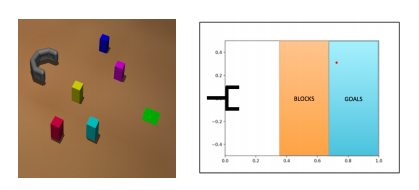
\includegraphics[scale=0.6]{MAESN_05.PNG}
	\centering
	\caption{Robotic Manipulation}
	\label{MAESN}
\end{figure}

In Wheeled Locomotion, a wheeled robot should move to different randomized goal locations with coherent exploration strategies.
\begin{figure}[H]
	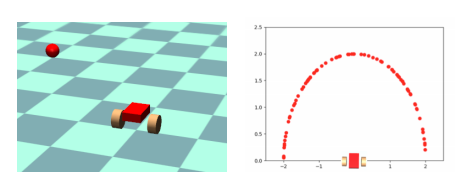
\includegraphics[scale=0.53]{MAESN_06.PNG}
	\centering
	\caption{Wheeled Locomotion}
	\label{MAESN}
\end{figure}

In Legged Locomotion, an ant walks to randomly placed goals, which requires carefully coordinated leg motions.
\begin{figure}[H]
	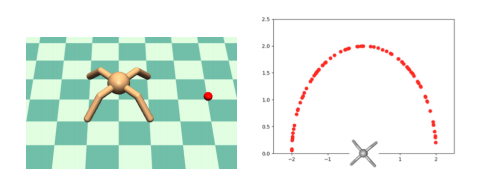
\includegraphics[scale=0.53]{MAESN_07.PNG}
	\centering
	\caption{Legged Locomotion}
	\label{MAESN}
\end{figure}
In the same time we compare MAESN with other 6 exploration approaches during meta-test on each task distribution, that are RL$^2$ [15], MAML, simply learning latent spaces without fast adaptation(LatentSpace), TRPO, REINFORCE, and training from scratch with VIME [16]. 

\begin{figure}[H]
	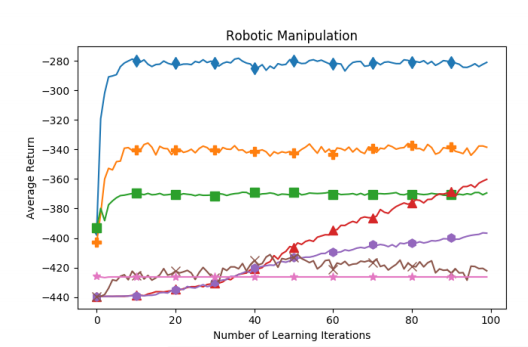
\includegraphics[scale=0.6]{MAESN_09.PNG}
	\centering
	\caption{results of Robotic Manipulation}
	\label{MAESN}
\end{figure}
\begin{figure}[H]
	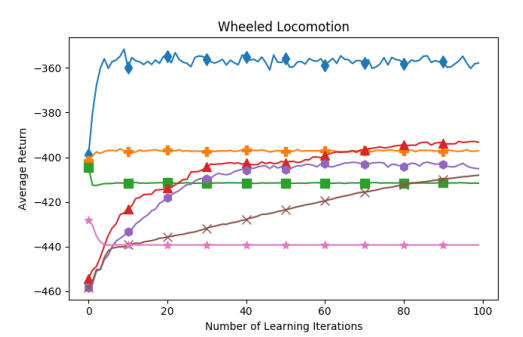
\includegraphics[scale=0.6]{MAESN_10.PNG}
	\centering
	\caption{results of Wheeled Locomotion}
	\label{MAESN}
\end{figure}
\begin{figure}[H]
	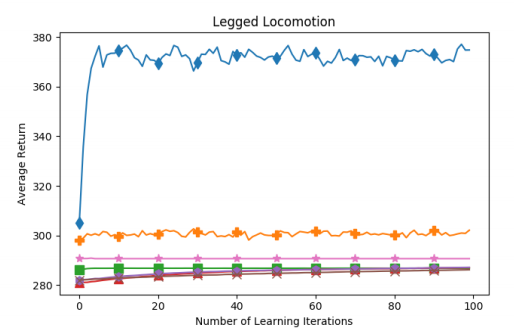
\includegraphics[scale=0.6]{MAESN_11.PNG}
	\centering
	\caption{results of Legged Locomotion}
	\label{MAESN}
\end{figure}
From the results of all exploration strategies we find that the latent variable based MAESN performs much better on new tasks compared to either prior meta-learning approaches or the methods learning from scratch, since MAESN is able to train latent space for fast adaptation.









